% !TEX encoding = UTF-8
% !TEX TS-program = pdflatex
% !TEX root = ../tesi.tex

\newgeometry{a4paper, left=30mm, right=30mm, top=5mm, bottom=30mm}
%**************************************************************
\chapter{Progettazione e codifica}
\label{cap:progettazione-codifica}
%**************************************************************

\noindent \intro{In questo capitolo vengono esposte le attività di progettazione e codifica del modulo di ottimizzazione}\\

%**************************************************************
\section{Architettura}
\label{sec:progettazione}
\noindent Prima di descrivere più in particolare l'algoritmo, è necessario
fornire un’idea dell’architettura sulla quale si basa l'intero progetto.
Di seguito è presentato uno schema ad alto livello di come sono strutturate le varie
componenti che formano il sistema.

\begin{figure}[!h] 
    \centering 
    \includegraphics[width=0.95\columnwidth]{architettura/architettura.pdf} 
    \caption{Architettura generale}
    \label{architettura-generale}
\end{figure}

\noindent Come si può notare in figura \ref{architettura-generale},
il flusso del sistema è circolare.
Si parte dal database, dal quale vengono estratti i dati di interesse dalle varie
tabelle. Successivamente viene fatto il pre-processing dei dati,
in modo tale da poter poi eseguire l'ottimizzazione solo su
ciò che è di interesse dell'analisi.
Viene effettuato il controllo dei vincoli al termine
dell'algoritmo così da generare
una soluzione ammissibile. Se si vuole effettuare una nuova
analisi è necessario estrarre nuovamente i dati dal
database ed eseguire nuovamente il ciclo. Questo è necessario
in quanto i dati all'interno del database possono variare
(esempio: prezzi, date di spedizione...).

\newpage

\newgeometry{a4paper, left=30mm, right=30mm, top=31mm, bottom=30mm}

\section{Funzionamento generale}
In questa sezione viene descritta una classica interazione dell'utente con il programma.
Nella figura \ref{diagramma-attivita-winform} si riassume il flusso delle interazioni.

\begin{figure}[!h] 
    \centering 
    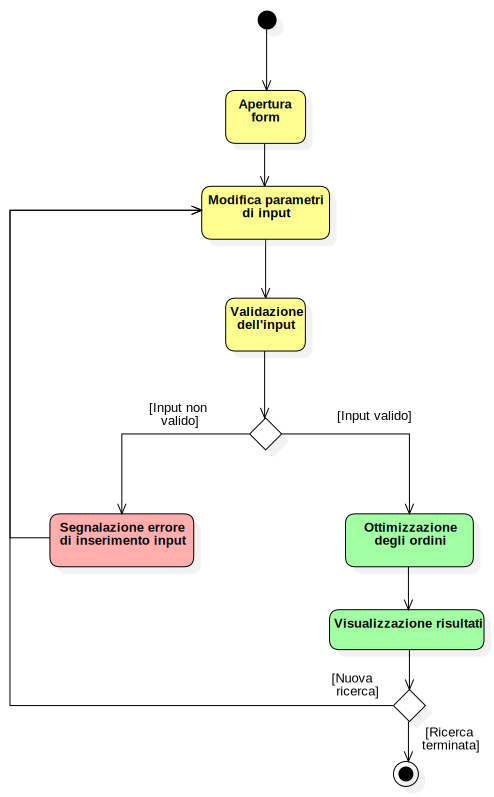
\includegraphics[scale = 0.75]{diagrammi attivita/Diagramma di attivita winform.pdf} 
    \caption{Diagramma di attività della WinForm}
    \label{diagramma-attivita-winform}
\end{figure}

\noindent L'utente, all'apertura della WinForm, modifica i parametri di input che sono:
\begin{itemize}
    \item data di previsione iniziale
    \item data di previsione finale
    \item metodo di risoluzione dei vincoli
\end{itemize}
\noindent Dopo aver scelto gli input, questi vengono validati in modo tale da bloccare anzitempo
l'esecuzione in caso di input errati.
Se la validazione va a buon fine allora l'algoritmo calcola la soluzione e vengono visualizzati i risultati.
A questo punto la ricerca può terminare oppure può continuare con la possibilità di variare i parametri di input.

%**************************************************************
\section{Tabu Search}
\label{sec:tabu-search}
\noindent Nella sezione §\ref{conclusione-studio-fattibilita}
riguardante lo studio di fattibilità è emerso come la tabu search
sia il giusto compromesso in termini di efficacia, efficienza
e complessità a livello implementativo.
In figura \ref{diagramma-attivita-tabu-search}
viene rappresentato il funzionamento generale dell'algoritmo.

\begin{figure}[!h] 
    \centering 
    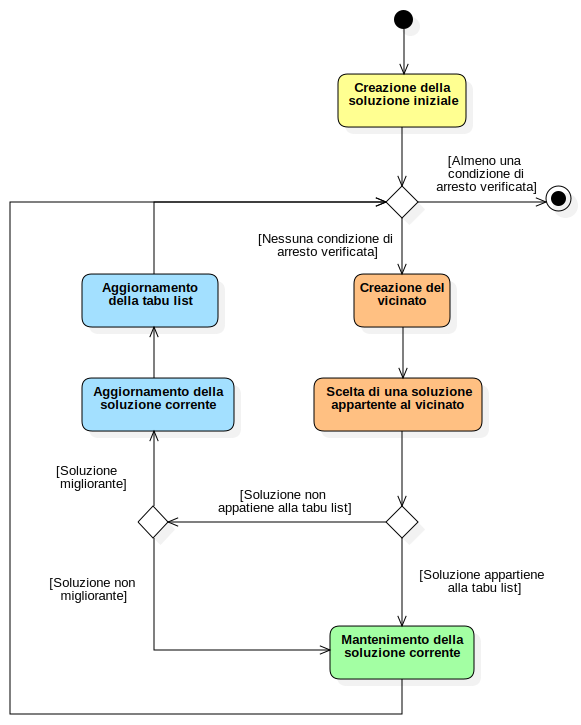
\includegraphics[width=0.8\columnwidth]{diagrammi attivita/diagramma attivita tabusearch.pdf} 
    \caption{Diagramma di attività della WinForm}
    \label{diagramma-attivita-tabu-search}
\end{figure}

%**************************************************************
\subsection{Rappresentazione della soluzione}
\label{sec:rappresentazione-della-soluzione}

%**************************************************************
\subsection{Soluzione iniziale}
\label{sec:soluzione-iniziale}

\begin{algorithm}
    \captionsetup{labelformat=empty}
    \caption{Pseudocodice soluzione iniziale - Algoritmo Greedy}
    \vspace{0.1cm}
    \hspace*{\algorithmicindent} \textbf{Input:} {$lista\_articoli$}, {$lista\_vincoli$}\\
    \hspace*{\algorithmicindent} \textbf{Output:} {$lista\_articoli\_opt$}
    \begin{algorithmic}[1]
        \Procedure{My\_Greedy\_Algorithm}{$lista\_articoli$, $lista\_vincoli$}
        \State {$l \gets lista\_vuota$}
        \State {$l_{tmp} \gets lista\_vuota$}
        \State $l_{cod\_art} \gets genera\_lista\_decisione(lista\_articoli)$
        \State $n_{cod\_art} \gets l_{cod\_art}.Length$
        \While {$count < n_{cod\_art}$}
            \State {$cod\_art \gets decisione(l_{cod\_art})$}
            \ForAll {$art \in lista\_articoli$}
                \State {$b \gets controllo\_vincoli(art$, $cod\_art$, $lista\_vincoli)$}
                \If {$b = true$}
                    \State Aggiungi $art$ a $l_{tmp}$
                \EndIf
            \EndFor
            \State {$count \gets count+1$}
        \EndWhile
        \State $l \gets filtra\_articoli\_per\_min(l_{tmp})$
        \State \Return $l$
        \EndProcedure
    \end{algorithmic}
\end{algorithm}

%**************************************************************
\subsection{Esplorazione del vicinato}
\label{sec:esplorazione-vicinato}

%**************************************************************
\subsection{Mosse}
\label{sec:mosse}

%**************************************************************
\subsection{Tabu List}
\label{sec:tabu-list}

%**************************************************************
\subsection{Funzione di valutazione}
\label{sec:funzione-valutazione}

%**************************************************************
\subsection{Condizioni di arresto}
\label{sec:condizioni-arresto}

%**************************************************************
\subsection{Controllo dei vincoli}
\label{sec:controllo-vincoli}

%**************************************************************
\section{Codifica}
\label{sec:codifica}

%**************************************************************
\subsection{Organizzazione dello sviluppo}
\label{sec:organizzazione-sviluppo}

%**************************************************************
\subsection{Log}
\label{sec:log}

%**************************************************************
\subsection{Problematiche riscontrate}
\label{sec:problematiche-riscontrate}

%**************************************************************
\subsection{Estensioni degli algoritmi}
\label{sec:estensioni-algoritmi}

\newpage

%**************************************************************
\section{Tecnologie e strumenti}
\label{sec:tecnologie-strumenti}

\noindent Di seguito viene esposta una panoramica delle tecnologie e degli strumenti utilizzati.
Sono stati tutti imposti da Ergon Informatica in quanto sono le tecnologie e gli strumenti
da loro impiegati per lo sviluppo software.\\
Per l’azienda le caratteristiche determinanti della scelta di queste tecnologie
sono riconducibili alle soddisfazione delle seguenti necessità e aspettative:
\begin{itemize}
    \item compatibilità con il sistema Ergdis;
    \item facilità di apprendimento;
    \item ampia disponibilità della documentazione;
    \item gradevolezza dell’interfaccia grafica.
\end{itemize}
Di seguito vegono presentate le tecnologie utilizzate.


\subsection*{C\#}
\begin{figure}[!h] 
    \centering 
    \includegraphics[scale = 0.04]{loghi/CSharpLogo.pdf} 
    \caption{Logo C\#}
 \end{figure}
\noindent C\# è un linguaggio di programmazione multi-paradigma orientato agli oggetti
sviluppato da Microsoft. La sua sintassi e struttura derivano da altri linguaggi nati
precedentemente, come C++, Java e Visual Basic.\\
C\# è progettato per essere compatibile con le classi e l’ambiente di compilazione
del framework .NET. Supporta astrazione, ereditarietà e polimorfismo
fornendo estensibilità e riusabilità del codice.
È stato ufficialmente approvato come standard dalla ECMA.\\
L'azienda, sebbene abbia sviluppato la maggior parte dei moduli
in Visual Basic, sta lentamente traducendo tutto in questo linguaggio.

\subsection*{Visual Studio 2019}
\begin{figure}[!h] 
    \centering 
    \includegraphics[scale = 0.75]{loghi/VisualStudio2019Logo.pdf} 
    \caption{Logo Visual Studio 2019}
 \end{figure}
\noindent Visual Studio 2019 è un ambiente di sviluppo integrato (IDE) fornito da Microsoft.
Permette lo sviluppo di software per computer, siti web, applicazioni web, servizi web
e applicazioni mobile. È compatibile con tutte le piattaforme di sviluppo
software Microsoft, quali Windows API e Windows Form.\\
Visual Studio 2019 supporta il refactoring del codice e intellisense, uno strumento per
l’autocompletamento del codice. Il debugger integrato funziona sia a
livello di codice sorgente che a livello di codice macchina. È compatibile anche con i sistemi di supporto per il controllo del codice,
come per esempio Subversion e Git.\\
Visual Studio 2019 supporta 36 differenti linguaggi di 
programmazione tra i quali C\#.

\subsection*{DevExpress}
\begin{figure}[!h] 
    \centering 
    \includegraphics[scale = 0.35]{loghi/DevExpressLogo.png}
    \caption{Logo DevExpress}
\end{figure}
\noindent DevExpress è una compagnia che produce strumenti di sviluppo software per
Visual Studio. In particolare crea estensioni che vengono utilizzate tramite Visual
Studio per velocizzare la scrittura di applicazioni. Gli strumenti da loro forniti sono
molteplici, in particolare hanno sviluppato controlli .NET di interfaccia utente (UI).
Questi ultimi rendono più semplice la creazione di ambienti grafici per applicazioni ed
elegante il risultato.

\subsection*{Informix}
\begin{figure}[!h] 
    \centering 
    
\includegraphics[scale = 0.04]{loghi/InformixLogo.pdf}
    \caption{Logo IBM Informix}
\end{figure}
\noindent IBM Informix è un prodotto di IBM. La base di dati Informix è usata in molte
applicazioni OLTP ad alto tasso di transazione che operano in vari settori tra cui anche quelli della produzione e dei trasporti.\\
L’Informix server supporta il modello relazionale ad oggetti che permette ad IBM di
offrire estensioni che permettono di effettuare interrogazioni per un dominio specifico
e archiviazioni per set di dati in maniera rapida ed efficiente.
É in grado di supportare sia SQL che NoSQL.

\subsection*{Git}
\begin{figure}[!h] 
    \centering 
    \includegraphics[scale = 0.4]{loghi/GitLogo.pdf}
    \caption{Logo Git}
\end{figure}
\noindent Git è uno strumento per il controllo di versione distribuito del codice sorgente delle repository.\\
Creato inizialmente per gestire le versioni del kernel Linux, al giorno d'oggi è uno dei principali
strumenti di versionamento del codice e di collaborazione tra gli sviluppatori.
